\pagebreak
\section{Html Presentation}
Now we need to convert the Entities we have into html.
First we create the index.jsp file, which is a simple form that has a field for the matriculation and two checks, one for each page, to choose what to generate: in this way, we can test both pages simultaneously (the real version would have two different buttons that redirects to two different pages).

\begin{figure}[H]
  \centering
  
\includegraphics[width=\columnwidth]{index.png}
  \caption{The starting page}
\end{figure}

The form will redirect to our servlet, which will call a special bean, HtmlElementEBJ, used to create the elements we need for our page. This bean will use the FacadeEJB to call its method, parse the results and transform them into a ready-to-use html element. This is known as Business Delegate: by dealing with the business implementation in this bean, we can free the client part from knowing the backend, instead of referencing FacadeEJB all across the frontend. The shown version uses a local FacadeEJB: we will see later how to convert it to a remote call.

\begin{lstlisting}[language=java, caption={Servlet doPost}]
    public void doPost(HttpServletRequest request, HttpServletResponse response) throws IOException {
      int matriculation;
      try {
        matriculation = Integer.parseInt(request.getParameter("matriculation"));
      } catch (NumberFormatException e) {
        response.sendRedirect("");
        return;
      }
      boolean showStudentPage = request.getParameter("studentPage") != null;
      boolean showAdvisoryPage = request.getParameter("advisoryPage") != null;

      String html = "";
      String name;
      try {
        name = "java:module/HtmlElementsEJB!it.marrocco.h2ejbdemo.ejb.HtmlElements";
        HtmlElements htmlElementsEJB = (HtmlElements) ServiceLocator.getService(name);

        if (showStudentPage) html += htmlElementsEJB.getStudentPageElement(matriculation);
        if (showAdvisoryPage) html += htmlElementsEJB.getAdvisoryPageElement(matriculation);
      } catch (NamingException e) {
        html += "<h1>" + e.getMessage() + "</h1>";
      }

      response.setContentType("text/html");
      PrintWriter out = response.getWriter();
      out.println("<html><head><title>Matriculation "+matriculation+"</title></head><body>");
      out.println(html);
      out.println("<a href='index.jsp'>Go back</a>");
      out.println("</body></html>");
      out.close();
    }
  \end{lstlisting}

\begin{lstlisting}[language=java, caption={HtmlElementsEJB}]
    @Stateless
    @Local(HtmlElements.class)
    public class HtmlElementsEJB implements HtmlElements{
      Facade facadeEJB;
      public void ejbCreate() {
        try {
          facadeEJB = (Facade) ServiceLocator.getService("java:module/FacadeEJB!it.marrocco.h2ejbdemo.ejb.Facade");
        } catch (NamingException e) {
          throw new RuntimeException(e);
        }
      }
  
      @Override
      public String formatStudentEntity(StudentEntity s) {
        return "<h1>" + s.getSurname() + " " + s.getName() + " (" + s.getMatriculation() + ")</h1>";
      }
  
      @Override
      public String getStudentPageElement(int matriculation) {
        StudentEntity s = facadeEJB.getSingleStudent(matriculation);
        if (s == null) return "<h1>Student was not found</h1>";
        String html = formatStudentEntity(s);
        html += "<h2>Courses:</h2>";
        try {
          html += "<ul>";
          List<StudentCourseEntity> sc = facadeEJB.getStudentCourses(matriculation);
          if (sc == null) return "<h1>Error getting the Student Courses</h1>";
          for (StudentCourseEntity c : sc) {
            html += "<li>" + c.getCourse().getName();
            if(c.getGrade() != null)
              html +=  " (grade = " + c.getGrade() + ")";
            html += "</li>";
          }
          html += "</ul>";
        } catch (Exception e ) {
          System.out.println("error: " + e.getMessage());
          html += "<h3>error<h3>";
        }
        return html;
    }

    @Override
    public String getAdvisoryPageElement(int matriculation) {
        StudentEntity s = facadeEJB.getSingleStudent(matriculation);
        if (s == null) return "<h1>Student was not found</h1>";
        String html = formatStudentEntity(s);
        html += "<h2>Advisors:</h2>";
        try {
          html += "<ul>";
          List<TeacherEntity> sc = facadeEJB.getStudentTeachers(matriculation);
          if (sc == null) return "<h1>Error getting the Student Teachers</h1>";
          for (TeacherEntity t : sc) {
            html += "<li>" + t.getSurname() + " " + t.getName() + "</li>";
          }
          html += "</ul>";
        } catch (Exception e ) {
          System.out.println("error: " + e.getMessage());
          html += "<h3>error<h3>";
        }
        return html;
    }
    }
  \end{lstlisting}

\begin{figure}[H]
  \centering
  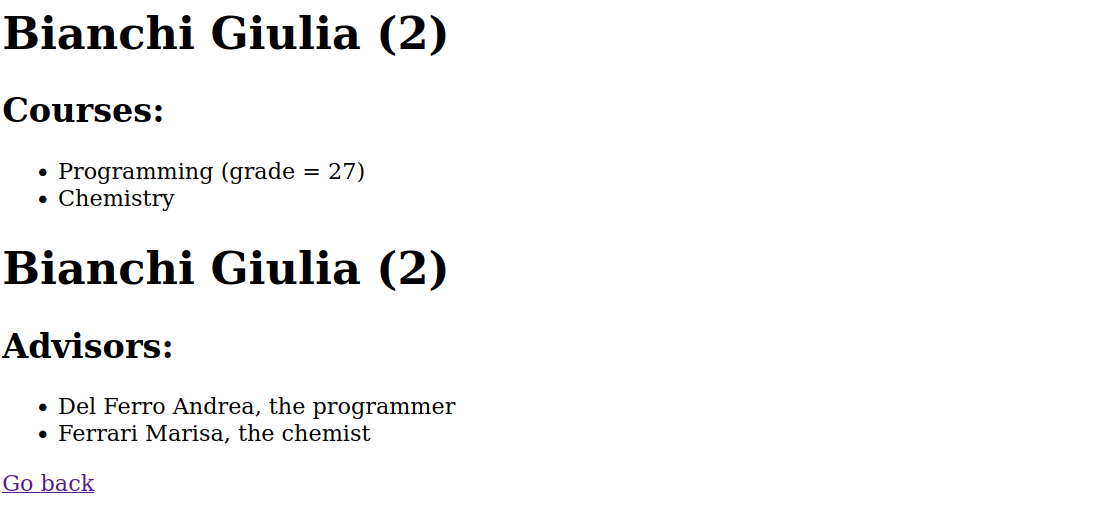
\includegraphics[width=\columnwidth]{full_page.png}
  \caption{The servlet page when both checks are set, showing both requested pages}
\end{figure}

\begin{figure}[H]
  \centering
  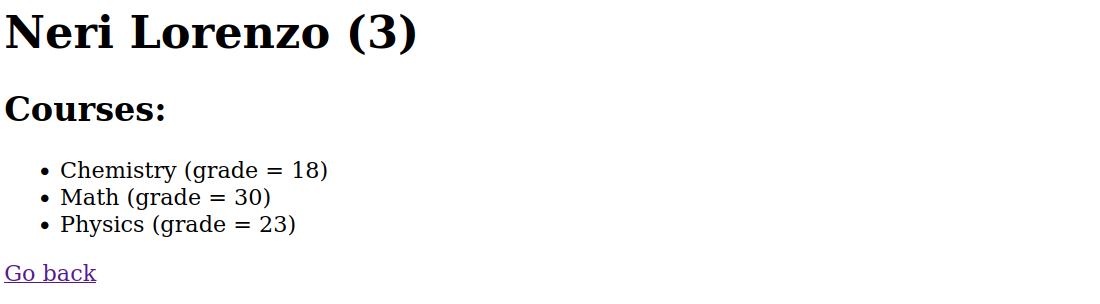
\includegraphics[width=\columnwidth]{only_one_page.png}
  \caption{The servlet page with only the courses page}
\end{figure}

\begin{figure}[H]
  \centering
  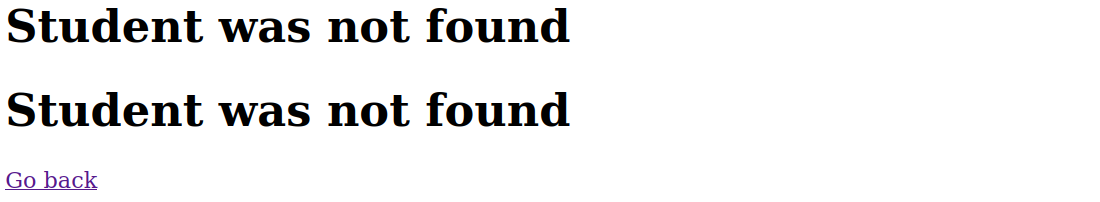
\includegraphics[width=\columnwidth]{no_student_found.png}
  \caption{The servlet page when a non existant student is searched}
\end{figure}

\pagebreak
\section{Client Tomcat}
The objective of this assignment was to separate in a distributed system the backend logic and the frontend presentation. Fortunately, this operation is not much complicated.
In the client server, what we need from the backend is:
\begin{itemize}
  \item  the entities, without the injection code;
  \item  the Facade interface, which will send us the serialized entities objects (DTO);
  \item  the HtmlElementsEJB, where we need to change the FacadeEJB lookup adress and substitute the method ebjCreate to a constructor;
  \item  the ServiceLocator, where in the context creation we need to add the Jndi properties to connect to the Wildfly server;
  \item  the index.jsp;
  \item  our servlet, where instead of using a lookup for the HtmlElementsEJB we need to instantiate the bean ourself in the code.
\end{itemize}

\begin{lstlisting}[language=java, caption={The new HtmlElementsEJB}]
    public class HtmlElementsEJB implements HtmlElements{
      Facade facadeEJB;
      public HtmlElementsEJB() {
        try {
          facadeEJB = (Facade) ServiceLocator.getService("ejb:/H2EJBDemo-1.0-SNAPSHOT/FacadeEJB!it.marrocco.h2ejbdemo.ejb.Facade");
        } catch (NamingException e) {
          System.out.println("Naming exception: " + e.getMessage());
          e.printStackTrace();
          throw new RuntimeException(e);
        }
      }
      // same methods as before
    }
  \end{lstlisting}

\begin{lstlisting}[language=java, caption={The new ServiceLocator}]
    public class ServiceLocator {
      private static HashMap<String, Object> cache;

      static {
        cache = new HashMap<String, Object>();
      }

      private static Properties getJndiProperties() {
        Properties jndiProperties=new Properties();
        jndiProperties.put(Context.INITIAL_CONTEXT_FACTORY, "org.wildfly.naming.client.WildFlyInitialContextFactory");
        jndiProperties.put(Context.PROVIDER_URL,"http-remoting://localhost:8080");
        return jndiProperties;
      }

      public static Object getService(String jndiName) throws NamingException {
        Object service = cache.get(jndiName);
        if (service == null) {
          InitialContext context = new InitialContext(getJndiProperties());
          service = context.lookup(jndiName);
          cache.put(jndiName, service);
        }
        return service;
      }
    }
  \end{lstlisting}

\begin{lstlisting}[language=java, caption={The new Servlet doPost}]
    public void doPost(HttpServletRequest request, HttpServletResponse response) throws IOException {
      // same parameters controlls as before
      String html = "";
      try {
        HtmlElements htmlElementsEJB = new HtmlElementsEJB();

        if (showStudentPage) html += htmlElementsEJB.getStudentPageElement(matriculation);
        if (showAdvisoryPage) html += htmlElementsEJB.getAdvisoryPageElement(matriculation);
      } catch (Exception e) {
        System.out.println("Error in fetching data");
        html += "<h1>Error in fetching data</h1>";
      }
      // same html creation as before
    }
  \end{lstlisting}
